This section presents an exploratory data analysis (EDA) of the drought impact database. The goal is to understand the characteristics of the dataset before it is used for predictive modelling. In particular, the analysis focuses on identifying temporal, spatial, and thematic patterns that may influence model development and performance.

The section begins with a temporal analysis of yearly trends, seasonality, and their relationship with meteorological drought conditions. Next, the spatial distribution of reported impacts is examined to identify potential geographical biases. Finally, the distribution and co-occurrence of drought impact types are analysed to better understand class imbalance and relationships between impact categories. The findings of this analysis are used to motivate modelling decisions in the following chapter.




\section{Temporal analysis}
\subsection{Volume}

Figure \ref{fig:yearly_volume} shows the yearly number of reported impacts between 2005 and 2025.
From 2005 to 2017, the number of reported impacts remained relatively low, with an average of about 234 impacts per year.
From 2018 onward, the number of reported impacts increased strongly, with an average of about 1,569 impacts per year (12,550 impacts in total; 80.5\% of the 2005--2025 corpus).
The year 2018 corresponds with an extreme drought event in the Netherlands, but the magnitude of the increase suggests that reporting practices may have changed after this period.
\begin{figure}[h!]
    \centering
    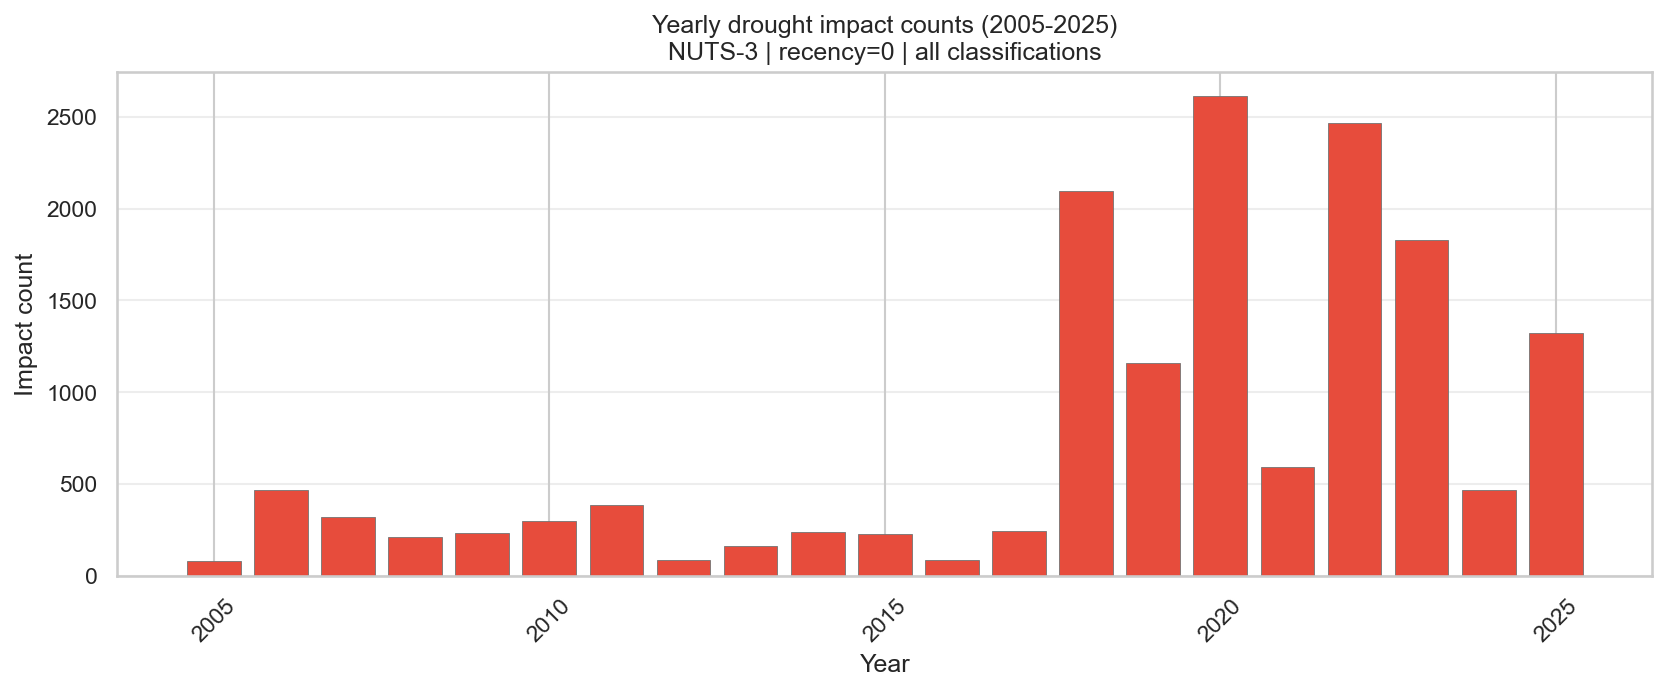
\includegraphics[width=0.98\linewidth]{figures/EDA/fig_yearly_volume.png}
    \caption{Yearly drought impact counts}
    \label{fig:yearly_volume}
\end{figure}
The increase occurred mainly between 2017 and 2018, where the number of reported impacts increased from 244 to 2,095.

Due to this large change, the periods before and after 2018 are treated as separate reporting periods in the remainder of this chapter.

\subsection{Meteorological context}



To provide meteorological context, the yearly number of reported drought impacts is compared with the KNMI national cumulative precipitation deficit on 30 September, a commonly used indicator of drought severity in the Netherlands.

The analysis is performed separately for the two reporting periods (2005--2017 and 2018--2025). Within each period, both the KNMI drought indicator and the yearly number of reported impacts are normalized using min-max scaling. The normalized values are then compared for each year. Years with an absolute difference greater than 0.40 are highlighted, indicating a large mismatch between the reported drought impacts and the meteorological drought indicator.

This threshold-based approach was chosen instead of a correlation coefficient because it is easier to interpret and does not rely on distributional assumptions such as normality.

Figure \ref{fig:meteo_comparision} presents the results. In the period 2005--2017, several years (2007, 2009, 2011, 2013, and 2016) show large differences between the normalized impact counts and the KNMI drought indicator. In contrast, no years exceed the same threshold during the 2018--2025 period.

\begin{figure}
    \centering
    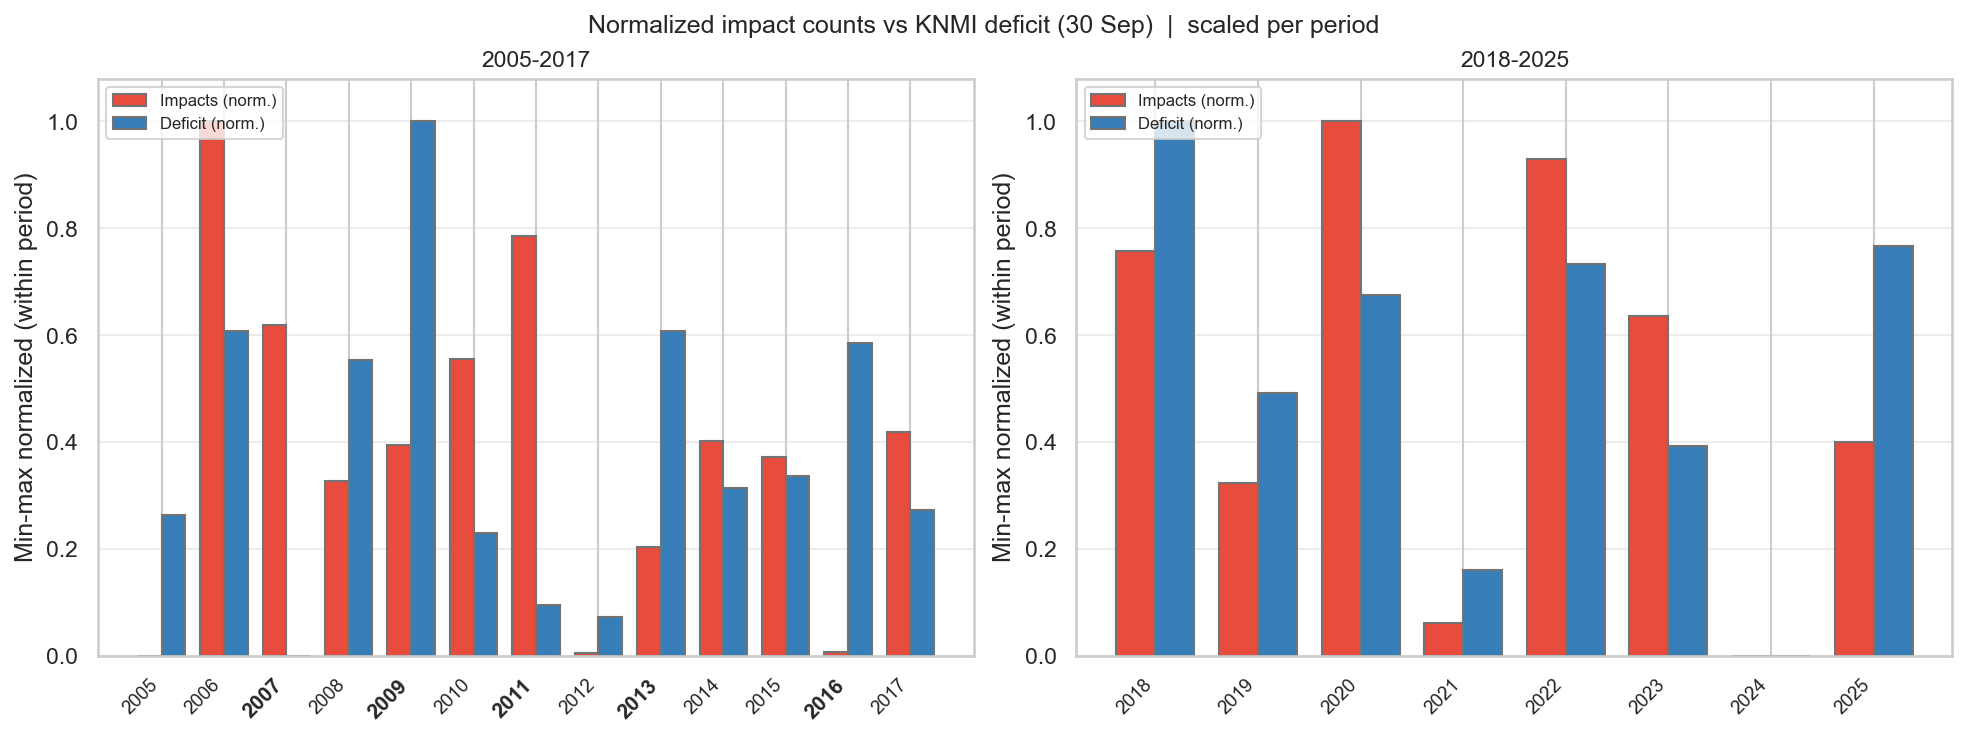
\includegraphics[width=1\linewidth]{figures/EDA/fig_meteo_comparison.png}
    \caption{Bold years mark large within-period mismatches between normalized impacts and KNMI 30-Sep deficit (2007, 2009, 2011, 2013, 2016); no year in 2018–2025 exceeds the same threshold.}
    \label{fig:meteo_comparision}
\end{figure}

These results suggest that the reported drought impacts align more closely with meteorological drought conditions after 2018 than before. For the pre-2018 period, the extracted news signal appears to be weaker and less consistent with the observed drought conditions. This does not imply that individual drought impacts or sectors cannot be modelled during this period. Instead, it suggests that the overall reporting signal is relatively weak, making it more difficult to distinguish years with different levels of drought severity.

One possible explanation is that drought impacts in the news were reported less consistently before 2018, resulting in a dataset with a lower signal-to-noise ratio. Consequently, the pre-2018 data should be interpreted with caution when used for predictive modelling. For this reason, the models developed in this thesis primarily focus on the 2018--2025 period, where the relationship between reported impacts and meteorological drought conditions appears to be more consistent.


\subsection{Monthly seasonality}

When aggregating impact mentions by publication month, a strong seasonal pattern is observed. Approximately 61\% of all impact mentions are published between May and September, while July and August together account for around one-third of the complete dataset. In contrast, the winter months December, January, and February together contain only around 13\% of all mentions. Figure \ref{fig:seasonality} shows this seasonality.

\begin{figure}
    \centering
    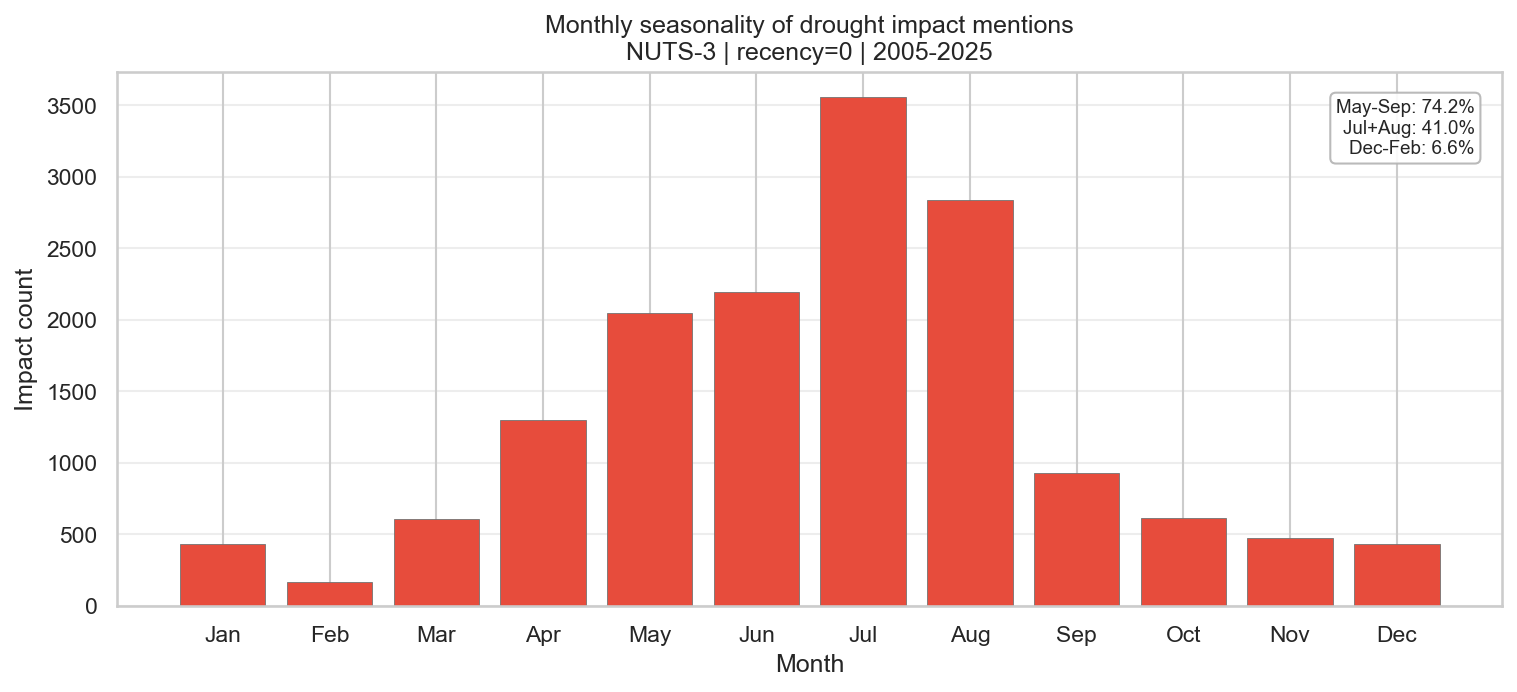
\includegraphics[width=1\linewidth]{figures/EDA/fig_monthly_seasonality.png}
    \caption{Monthly seasonality Drought impacts}
    \label{fig:seasonality}
\end{figure}

This seasonal pattern is partly consistent with drought processes, as summer conditions are associated with higher temperatures, increased evaporation, and greater water stress. However, the strong concentration of reports during summer may also indicate a reporting bias, where drought impacts are more frequently reported when they are more visible and receive more public attention.





\section{Spatial analysis}

Figure~\ref{fig:choropleth-nuts3} shows that a higher number of reported impacts is observed in regions with sandy soils. The five NUTS-3 regions with the highest reported impact totals are Achterhoek (797), Veluwe (715), Zuidoost-Noord-Brabant (709) and West-Noord-Brabant (592). These regions are characterised by intensive agriculture, sandy soils, and relatively shallow groundwater levels. Overig Zeeland (616) has high impacts because it mainly depends on rain water.

\begin{figure}[h!]
    \centering
    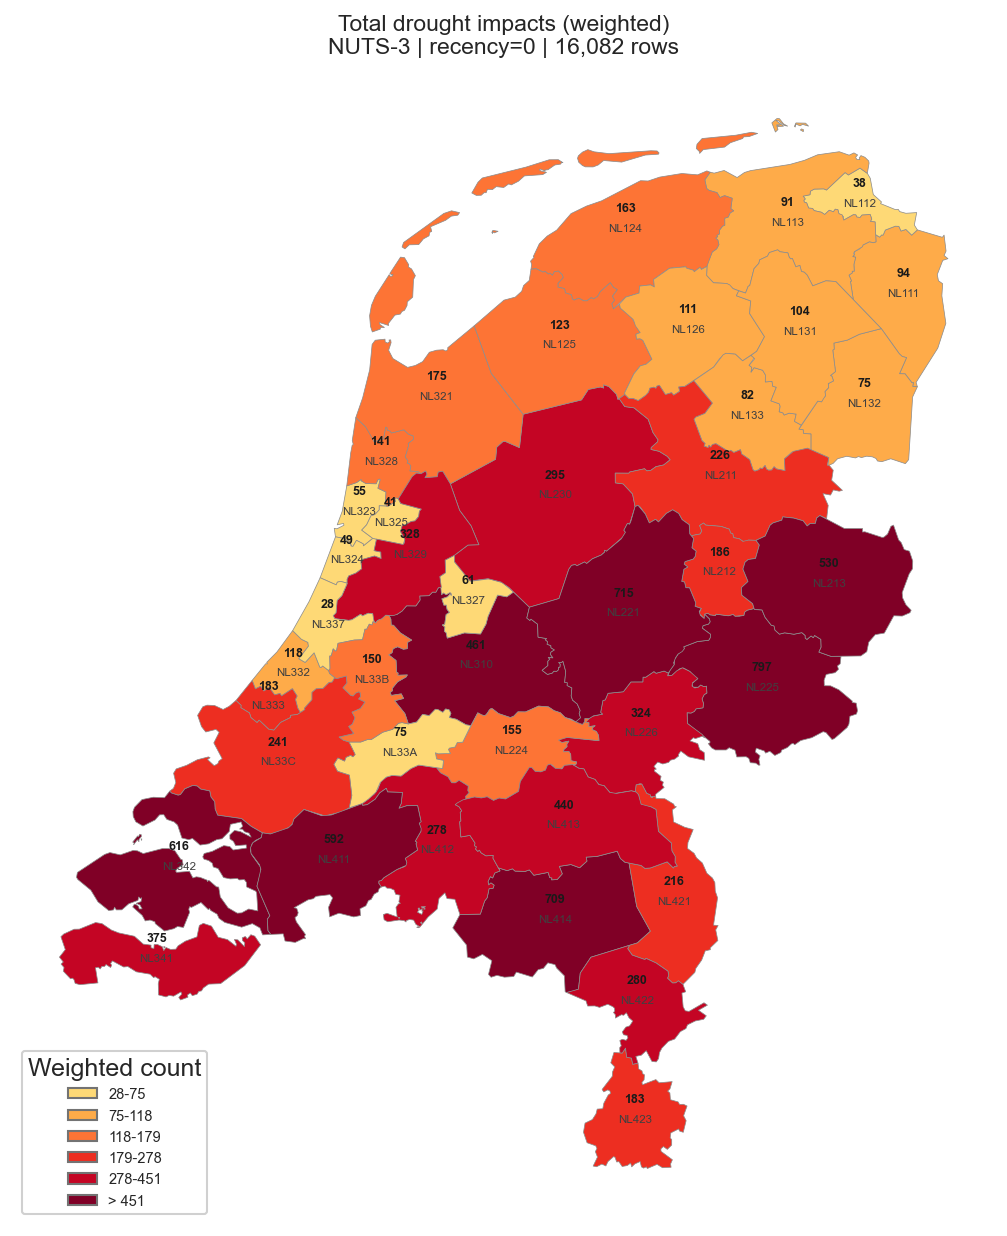
\includegraphics[width=0.5\linewidth]{figures/EDA/fig_choropleth_nuts3.png}
    \caption{Total weighted drought impact counts by NUTS-3 region (2005--2025; \texttt{recency\_in\_months}=0). Darker colours indicate higher impact totals; values shown on the map are region totals.}
    \label{fig:choropleth-nuts3}
\end{figure}

The lowest impact totals occur mainly in densely populated urban regions of the Randstad, such as Agglomeratie Leiden en Bollenstreek (28), Zaanstreek (41), and Agglomeratie Haarlem (49). Since these regions are not characterised by low population density, the spatial distribution of reported drought impacts appears to be more strongly related to land use and hydrogeological conditions than to population density or media presence.

This suggests that variables such as population density, which are commonly used in drought impact studies at coarser spatial resolutions, may have limited explanatory power for this dataset. Instead, land use and hydrological characteristics may be more relevant predictors of drought impacts in the Netherlands.

Additionally, the specific geographical characteristics of the Netherlands should be considered. A large part of the country is located below sea level, meaning that elevation and water management systems may influence drought vulnerability. For example, maintaining groundwater levels in elevated sandy regions can be more challenging than in lower-lying areas where water can be supplied more easily through existing infrastructure.

Based on these observations, the selection of model input variables should consider the specific Dutch context. Variables related to land use, soil type, groundwater availability, and elevation may provide more relevant information for drought impact modelling than variables commonly applied in other regions.

\section{Impact characteristic's}

\subsubsection{Sector distribution}

Grouping the 19 impact classifications into their six thematic categories
gives the following weighted distribution: agriculture 5,093 (36.2\%),
water 4,253 (30.2\%), ecosystem 2,450 (17.4\%), fire/heat 1,307 (9.3\%),
economy 522 (3.7\%), and social 460 (3.3\%). Agriculture and water together
account for two-thirds of all reported impacts. The overall sector distribution is shown in Figure \ref{fig:class_distribution}, representing a highly imbalanced dataset across sectors.

\begin{figure}[h!]
    \centering
    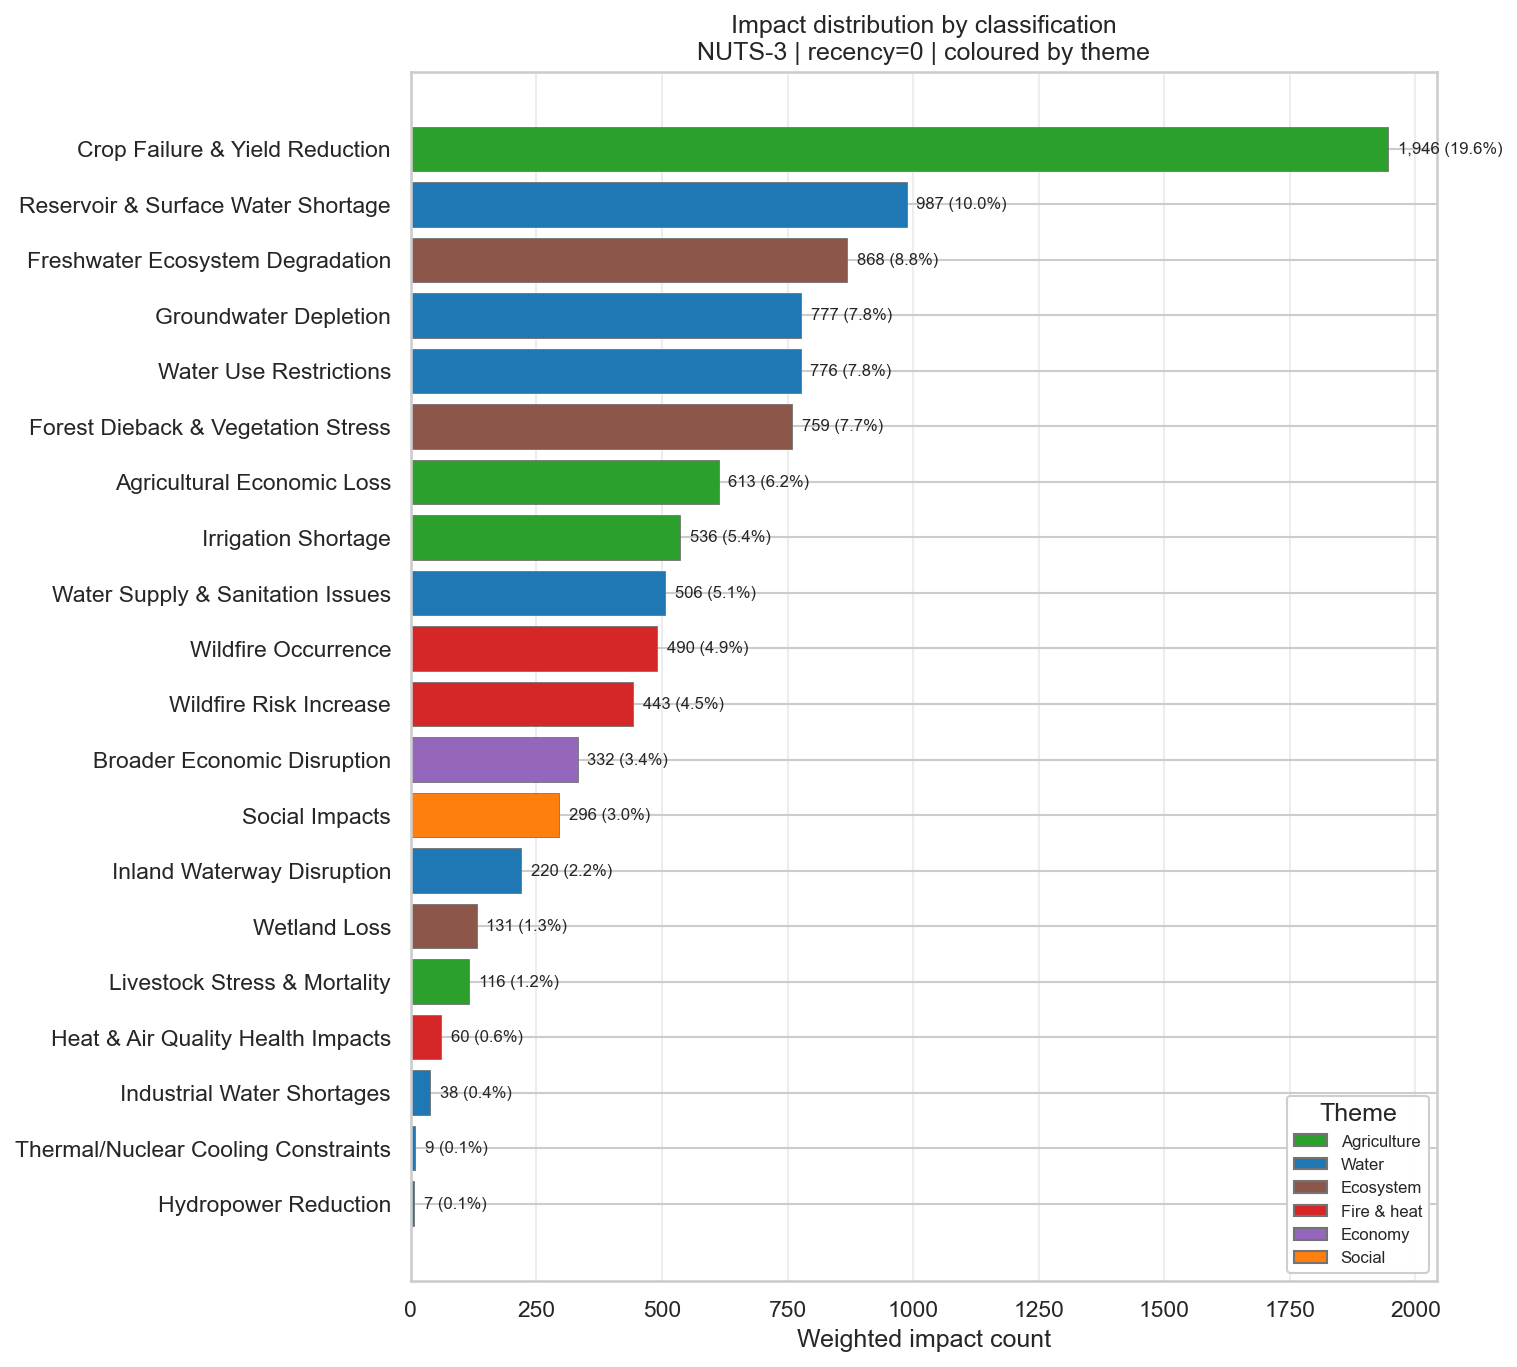
\includegraphics[width=0.85\linewidth]{figures/EDA/fig_class_distribution.png}
    \caption{The distribution of drought impact across all 19 classes.}
    \label{fig:class_distribution}
\end{figure}

\subsection{Co-occurrence signals}

Some impacts frequently co-occur and are often reported together. In this analysis, impact co-occurrence is defined as impacts that co-occur \textbf{within the same news-article}. Co-occurrence patterns in this dataset can be caused by the following mechanism.  Impacts are connected through underlying causal chains. For example, a reduction in crop yield can lead to agricultural economic losses.

Figure \ref{fig:cooccurrence_article_arc} shows the co-occurrence patterns between different impact types. From these patterns, several potential impact chains can be identified:

\begin{figure}
    \centering
    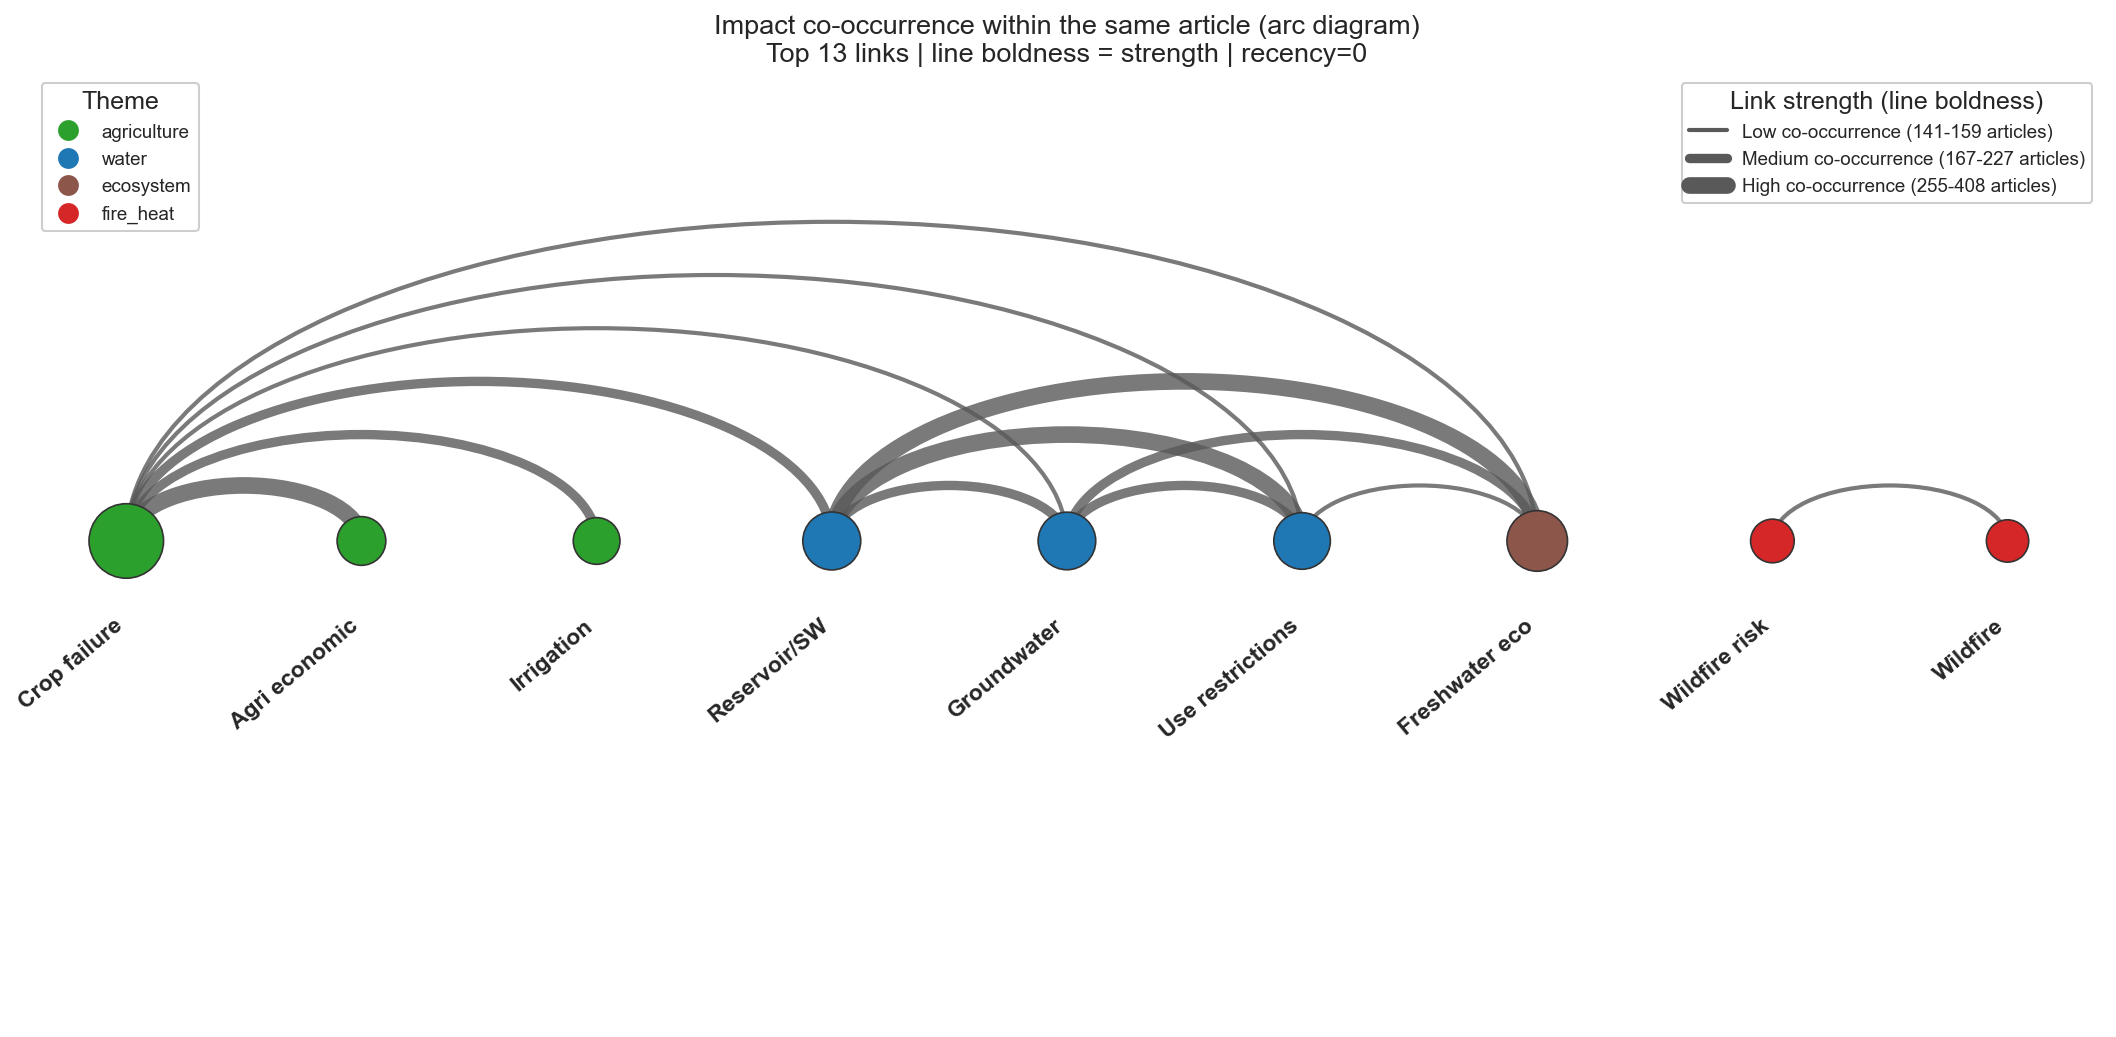
\includegraphics[width=1\linewidth]{figures/EDA/fig_cooccurrence_article_arc.png}
    \caption{Co-occurrence of top 13 impact links}
    \label{fig:cooccurrence_article_arc}
\end{figure}

\begin{itemize}
    \item Wildfire risk increase $\rightarrow$ wildfire occurrence
    \item Irrigation shortage $\rightarrow$ crop yield loss $\rightarrow$ agricultural economic loss
    \item Surface water shortage / groundwater shortage $\rightarrow$ water use restrictions / freshwater ecosystem degradation
\end{itemize}

These co-occurrence signals suggest that drought impacts are not independent events but can form connected chains. This information could potentially be used to simplify the modelling problem in several ways.

One option is to predict complete impact chains instead of individual impact classes. In this approach, an impact chain would become the prediction target rather than a single impact type. A second option is to focus on the beginning of these chains and model the occurrence of key initiating impacts, such as irrigation shortages, wildfire risk increases, or surface water shortages.

A third possibility is to focus on the relationships between impacts rather than predicting impacts directly. For example, instead of predicting when a water shortage occurs, a model could predict under which conditions a water shortage leads to water use restrictions. This would shift the modelling approach from predicting impacts towards modelling the links between impacts.

However, this type of causal impact modelling is likely already addressed in more specialised domain models developed for specific applications. A potential research direction inspired by the observed co-occurrence patterns is the use of Bayesian networks, which can explicitly represent relationships between variables and causal dependencies. This could provide an alternative to more commonly used machine learning approaches, within IBF such as random forests, which primarily model statistical relationships without explicitly representing causal structures. An other potential research venue could be using an causal random forest model, where we add causal rules to our random forest model.

\section{Implications for predictive modelling}

The exploratory data analysis highlights several characteristics of the drought impact database that should be considered during model development.

First, the temporal analysis identified a clear distribution shift after 2018. The stronger relationship between reported impacts and meteorological drought conditions suggests that the period 2018--2025 provides a more consistent training dataset than the earlier years. As a result, the predictive models developed in this thesis focus primarily on this period.

Second, the spatial analysis indicates that reported impacts are concentrated in agricultural regions with sandy soils. This suggests that variables describing land use, soil type, groundwater conditions, and elevation are likely to be more informative than population-based variables alone. The Dutch landscape differs from many previous drought impact studies, so feature selection should account for these regional characteristics.

Third, the impact distribution is highly imbalanced, with agriculture and water-related impacts dominating the dataset. This class imbalance should be considered during both model training and evaluation, as models may otherwise favour the largest classes.

Finally, the co-occurrence analysis shows that drought impacts sometimes occur in connected impact chains rather than as isolated events. Although this thesis predicts individual impact classes, these relationships suggest several directions for future work, including modelling impact chains directly or using causal machine learning methods such as Bayesian networks or causal random forests.

Together, these findings provide the basis for the feature selection and modelling choices described in the next chapter.



% This has to do with the underlying impact signals, but also with the way the llmn extract's the data. In our current str


% Some impacts co-occur alot, and some specif impcats do not co-occur alot. This has to do with the underlying procces in the impacts themeselves. To validate the database, and construct sort of an impact chain graph using network anlysis, we can create impact chains, to validate and visuliaze how the data is co-occuring alot. 

% The first step is to build an co-occurence matrix, what impact's co-occur alot, and how often do they co-occur. The question we want to anwser what drought impact do often co-occur together, and in what dirrection do they corruc? Then we have to add another constrained we want to make an directed graph, so that we can sort of visuliaze what impact's, lead to other impacts. 



% Building upon impact chan theory described in Section \ref{sec:impact_chain_theory}. 

















% ----------------------------

% \section{Research outputs: profiling the drought impact database}
% \label{sec:research-outputs}

% \subsection{Database overview}
% \label{subsec:db-overview}

% The database underlying this thesis is built from Dutch news articles
% processed by an LLM extraction pipeline, which identifies individual
% drought-impact mentions and assigns each one a location, an impact
% classification, a severity score, and a confidence score. Because a single
% article frequently reports several distinct impacts (e.g. a article about
% low river levels may simultaneously mention shipping disruption, water
% quality problems, and drinking-water concerns), it is important to
% distinguish two different units of analysis throughout this chapter:
% \emph{articles} (source documents) and \emph{impact mentions} (individual
% extracted impact statements, the unit the classifier is ultimately trained
% on).

% The full extraction output contains 48,444 impact mentions drawn from
% 15,318 unique articles (an average of 3.16 impact mentions per article),
% published between August 2004 and June 2026. Of these mentions, 22,658
% (46.8\%) could be geocoded precisely to one of the 40 Dutch NUTS-3 regions;
% the remainder refer to locations outside the Netherlands (32.3\%), resolve
% only to the country level (8.9\%), or could not be geocoded at all (12.0\%).
% This chapter focuses on the NUTS-3-resolvable subset, which spans 6,489
% unique articles and covers all 40 NUTS-3 regions and all 12 NUTS-2 provinces
% in the Netherlands. Within this subset, the average article mentions 1.85
% distinct impact classifications, and just over half of all articles
% (52.5\%) report more than one type of impact --- an early indication that
% drought impacts are rarely reported in isolation (see
% Section~\ref{subsec:impact-characteristics}).

% Impacts are grouped into 19 fine-grained classifications spanning six
% thematic groups: agriculture, water, ecosystem, fire/heat, economy, and
% social. Table~\ref{tab:db-overview} summarises the key scope statistics for
% the NUTS-3 subset used throughout the remainder of this chapter.

% \begin{table}[htbp]
%     \centering
%     \caption{Scope of the drought impact database (NUTS-3-resolvable subset).}
%     \label{tab:db-overview}
%     \begin{tabular}{lr}
%         \toprule
%         Quantity & Value \\
%         \midrule
%         Impact mentions (rows) & 22{,}658 \\
%         Unique source articles & 6{,}489 \\
%         Weighted impact count (mention-weighted) & 14{,}085 \\
%         Time period covered & 2004--2026 (bulk: 2005--2025) \\
%         NUTS-3 regions represented & 40 / 40 \\
%         NUTS-2 provinces represented & 12 / 12 \\
%         Impact classifications & 19 (6 thematic groups) \\
%         Articles reporting $>1$ impact type & 52.5\% \\
%         \bottomrule
%     \end{tabular}
% \end{table}

% \subsection{Temporal analysis}
% \label{subsec:temporal-analysis}

% \subsubsection{Yearly trends}

% \begin{figure}[htbp]
%     \centering
%     \includegraphics[width=0.85\textwidth]{images for report 2/bar_total_impacts_over_time.png}
%     \caption{Total reported drought impacts per year, 2005--2025.}
%     \label{fig:yearly-trend}
% \end{figure}

% Figure~\ref{fig:yearly-trend} shows annual impact counts restricted to
% 2005--2025. Between 2005 and 2017, yearly totals fluctuate between 121 and
% 578 (mean $\approx$ 325/year, total 4,227 impacts). From 2018 onward, annual
% totals jump to the low thousands (total 17,842 impacts over 2018--2025,
% mean $\approx$ 2,230/year) --- a step-change of roughly 4.2x in the average
% reporting rate, occurring almost entirely within a single year (2017: 376
% $\rightarrow$ 2018: 3,333). This shape --- an abrupt jump rather than a
% gradual ramp --- is the basis for treating 2005--2017 and 2018--2025 as two
% distinct reporting regimes for the remainder of this chapter.

% \subsubsection{Monthly seasonality}

% Aggregating impact mentions by publication month (full corpus, all
% geocoding levels) reveals a strong seasonal signal: 61\% of all impact
% mentions are published between May and September, with July (8,398
% mentions) and August (7,328) alone accounting for over a third of the
% entire corpus. The winter months are comparatively quiet: December,
% January, and February together account for only 13.5\% of mentions.
% \emph{[Figure to add: monthly histogram of impact mentions, currently not
% in the notebook --- can be generated from \texttt{publication\_date.dt.month}
% grouped counts.]}

% This pattern is only partly explained by actual drought physics. Summer is
% indeed when soil-moisture deficits, low river levels, and visible crop
% stress peak in the Netherlands, so some seasonality is expected. But the
% sharpness of the July/August spike also reflects a media-attention effect:
% drought is most newsworthy when it is visually and physically salient (heat,
% visible crop damage, low water levels for recreation), whereas slower-onset
% impacts such as groundwater depletion or ecosystem stress that persist into
% autumn and winter are comparatively under-reported once the summer news
% cycle ends. This is a second, independent reporting bias --- distinct from
% the year-level step-change --- that should be considered when interpreting
% month-level patterns in the data.

% \subsubsection{Relation to major drought years}

% The years with the highest impact counts in the post-2018 regime --- 2018,
% 2020, and 2022 --- correspond to the years widely documented as the most
% severe recent Dutch droughts, all part of the well-known cluster of dry
% summers between 2018 and 2022. This qualitative alignment is quantified
% formally in Section~\ref{subsec:meteo-context}.

% \subsubsection{Discussion of reporting bias}

% Taken together, the yearly and monthly patterns above indicate that the
% database's temporal structure is shaped as much by \emph{when and how
% drought gets reported} as by the underlying meteorological signal. The
% 2018 step-change most plausibly reflects a genuine shift in reporting
% volume/consistency (e.g. broader media and institutional attention
% following the record 2018 drought) rather than a sixfold increase in actual
% drought incidence in a single year. Similarly, the summer concentration of
% reports reflects newsworthiness as much as it reflects the physical timing
% of drought onset. Both biases matter directly for later chapters: any
% model trained on raw report volume as a proxy for drought intensity is, in
% part, learning a media-attention signal.

% \subsection{Spatial analysis}
% \label{subsec:spatial-analysis}

% \subsubsection{NUTS-2 / NUTS-3 maps}

% \begin{figure}[htbp]
%     \centering
%     
\includegraphics[width=0.85\textwidth]{outputs/eda_heatmaps/choropleth_total_impacts.png}
%     \caption{Total reported drought impacts per NUTS-3 region (weighted counts).}
%     \label{fig:choropleth-nuts3}
% \end{figure}

% At NUTS-3 resolution (Figure~\ref{fig:choropleth-nuts3}), impact reporting
% is concentrated in a relatively small number of regions. At the coarser
% NUTS-2 level, the concentration is still visible: three provinces ---
% Gelderland (2,660 weighted impacts), Noord-Brabant (2,656), and Overijssel
% (1,542) --- together account for 48.7\% of all weighted impacts, despite
% being only 3 of the Netherlands' 12 NUTS-2 provinces.
% \emph{[Figure to add: a NUTS-2 choropleth analogous to
% Figure~\ref{fig:choropleth-nuts3}, aggregating the existing NUTS-3 output up
% one administrative level --- not yet generated in the notebook.]}

% \subsubsection{Regional hotspots}

% The five NUTS-3 regions with the highest reported impact totals are
% Achterhoek (1,067), Veluwe (973), Zuidoost-Noord-Brabant (930), Overig
% Zeeland (928), and Twente (812) --- all agriculturally intensive areas on
% sandy soils with shallow groundwater tables. The lowest totals occur in
% dense, urbanised parts of the Randstad: Agglomeratie Leiden en
% Bollenstreek (43), Zaanstreek (53), and IJmond (70). Since these low-count
% regions are not low-population --- if anything the opposite --- the spatial
% pattern looks like a land-use/hydrogeology signal rather than a
% population- or media-density signal.

% \subsubsection{Density of impacts}

% The counts and maps above are absolute totals, not normalised by region
% size or population, so they should not yet be read as "risk density." A
% fair density comparison would divide each region's weighted impact count by
% its agricultural area (to test the land-use hypothesis) and, separately, by
% its population (to test whether the low urban counts genuinely reflect a
% reporting gap rather than a lower urban exposure to drought).
% \emph{[Analysis to add: per-km\textsuperscript{2} and per-capita normalised
% choropleths --- requires joining NUTS-3 area/population figures, e.g. from
% CBS or Eurostat, not currently in the notebook.]} Until this is done, the
% "hotspot" language in this section should be understood as a statement
% about reporting volume, not confirmed drought risk density.

% \subsection{Impact characteristics}
% \label{subsec:impact-characteristics}

% \subsubsection{Sector distribution}

% Grouping the 19 impact classifications into their six thematic categories
% gives the following weighted distribution: agriculture 5,093 (36.2\%),
% water 4,253 (30.2\%), ecosystem 2,450 (17.4\%), fire/heat 1,307 (9.3\%),
% economy 522 (3.7\%), and social 460 (3.3\%). Agriculture and water together
% account for two-thirds of all reported impacts, consistent with the
% regional pattern in Section~\ref{subsec:spatial-analysis}: both the
% sectoral mix and the spatial hotspots point toward the same underlying
% driver, namely agriculturally exposed, sandy-soil regions.

% \subsubsection{Cascading impacts and impact chains}

% Because 52.5\% of articles report more than one impact type, it is possible
% to treat co-occurring classifications within the same article as a proxy
% for cascading impact chains. Table~\ref{tab:cooccurrence} lists the most
% frequently co-occurring classification pairs within a single article.

% \begin{table}[htbp]
%     \centering
%     \caption{Most frequent co-occurring impact-classification pairs within the same article (NUTS-3 subset, $n=6{,}489$ articles).}
%     \label{tab:cooccurrence}
%     \begin{tabular}{lr}
%         \toprule
%         Co-occurring pair & Articles \\
%         \midrule
%         Agricultural Economic Loss $\leftrightarrow$ Crop Failure \& Yield Reduction & 661 \\
%         Freshwater Ecosystem Degradation $\leftrightarrow$ Reservoir \& Surface Water Shortage & 358 \\
%         Crop Failure \& Yield Reduction $\leftrightarrow$ Irrigation Shortage & 325 \\
%         Reservoir \& Surface Water Shortage $\leftrightarrow$ Water Use Restrictions & 290 \\
%         Freshwater Ecosystem Degradation $\leftrightarrow$ Groundwater Depletion & 289 \\
%         Groundwater Depletion $\leftrightarrow$ Reservoir \& Surface Water Shortage & 240 \\
%         Crop Failure \& Yield Reduction $\leftrightarrow$ Groundwater Depletion & 214 \\
%         Groundwater Depletion $\leftrightarrow$ Water Use Restrictions & 207 \\
%         Wildfire Occurrence $\leftrightarrow$ Wildfire Risk Increase & 180 \\
%         \bottomrule
%     \end{tabular}
% \end{table}

% Two distinct chains emerge from this table. The first is an
% agricultural chain: \emph{Crop Failure} co-occurs strongly with
% \emph{Irrigation Shortage} and \emph{Agricultural Economic Loss}, tracing a
% direct physical impact through to its economic consequence. The second is a
% water-system chain: \emph{Groundwater Depletion}, \emph{Reservoir \&
% Surface Water Shortage}, \emph{Freshwater Ecosystem Degradation}, and
% \emph{Water Use Restrictions} form a tightly interconnected cluster,
% consistent with a single hydrological cause propagating through surface
% water, groundwater, ecosystems, and policy response almost simultaneously
% within the same article. \emph{[Figure to add: a co-occurrence heatmap or
% network diagram of the full classification pair-count matrix would make
% this pattern easier to read than the table above.]}

% \subsubsection{Direct versus indirect impacts}

% Using the thematic grouping as a rough proxy --- treating economy and
% social impacts as downstream/indirect consequences, and
% agriculture/water/ecosystem/fire-heat impacts as direct physical
% consequences --- indirect impacts make up only 7.0\% of weighted mentions
% (982 of 14,085), against 93.0\% direct. This imbalance is worth stating
% explicitly: the database is overwhelmingly composed of \emph{direct}
% physical drought impacts, and the economic and social consequences of
% drought are comparatively rarely captured as a distinct, separately
% reported category, even though the co-occurrence analysis above shows they
% are frequently mentioned alongside a direct impact in the same article.

% \subsection{Meteorological context}
% \label{subsec:meteo-context}

% \begin{figure}[htbp]
%     \centering
%     \includegraphics[width=\textwidth]{images for report 3/timeseries_total_impacts.png}
%     \caption{Yearly impact counts versus KNMI cumulative precipitation deficit (30 September), shown separately per reporting regime with independent scaling.}
%     \label{fig:meteo-comparison}
% \end{figure}

% To test whether reported impact volume tracks actual meteorological drought
% severity, yearly impact counts (2005--2025) were compared against the KNMI
% national cumulative precipitation deficit as of 30 September --- a standard
% Dutch drought-severity indicator. The relationship differs sharply between
% the two reporting regimes identified in
% Section~\ref{subsec:temporal-analysis}:

% \begin{itemize}
%     \item \textbf{2005--2017:} Pearson $r = -0.02$ ($p = 0.87$), Spearman
%     $\rho = -0.05$ ($p = 0.87$) --- no detectable relationship between
%     yearly impact counts and the deficit.
%     \item \textbf{2018--2025:} Pearson $r = 0.78$ on raw counts (log-scaled:
%     $r = 0.84$, $p = 0.01$), Spearman $\rho = 0.60$ ($p = 0.12$) --- a
%     clear positive relationship, though the sample is small ($n=8$ years)
%     and statistical power is limited.
% \end{itemize}

% This is a striking result: reported impact volume is essentially unrelated
% to physical drought severity before 2018, but becomes a reasonably good
% proxy for it afterward. This is consistent with the reporting-regime
% interpretation from Section~\ref{subsec:temporal-analysis} --- before 2018,
% reporting was too sparse and inconsistent for its year-to-year variation to
% reflect real conditions; from 2018 onward, with a larger and more
% consistent volume of reporting, the aggregate signal starts to behave like
% a genuine (if noisy) drought indicator. A practical implication is that the
% pre-2018 subset should not be relied upon as ground truth for drought
% severity, while the post-2018 subset can be used with more confidence,
% subject to the caveats below.

% \subsubsection{Lead/lag relationships}

% A simple one-year-lag check (this year's impact count against last year's
% deficit) across the full 2005--2025 series gives $r = 0.23$ --- weak, and
% likely dominated by the level shift between regimes rather than a genuine
% lag effect. A within-regime lag analysis (particularly for 2018--2025) would
% require more years of data than are currently available to be conclusive,
% and should be revisited once more years accumulate.

% \subsubsection{Other meteorological variables}

% This comparison currently uses only the KNMI 30-September cumulative
% deficit. The processed meteorological dataset
% (\texttt{meteo\_nuts3\_monthly.parquet}, Chapter~7) also contains monthly
% SPEI-12 and, potentially, groundwater/soil-moisture fields at NUTS-3
% resolution, which would allow the comparison in this section to be repeated
% at regional rather than national level. \emph{[Analysis to add: NUTS-3-level
% correlation between weighted impact counts and local SPEI-12/groundwater
% anomalies, to test whether the national-level correlation above also holds
% regionally, or whether it is driven by a handful of high-volume regions.]}

% \subsection{Implications for predictive modelling}
% \label{subsec:modelling-implications}

% The patterns documented in this chapter translate into five concrete
% constraints that should inform how this database is used as training data
% in later chapters:

% \begin{enumerate}
%     \item \textbf{Temporal imbalance.} 79\% of all NUTS-3-resolvable impact
%     mentions (17,842 of 22,658) fall in 2018--2025, against 21\% in
%     2005--2017. Any temporal split or cross-validation scheme must account
%     for this, e.g. by stratifying by period rather than by simple random
%     year holdout.
%     \item \textbf{Spatial imbalance.} Just three NUTS-2 provinces account
%     for 48.7\% of weighted impacts, and the lowest-reporting NUTS-3 regions
%     have roughly 25x fewer impacts than the highest. A model evaluated only
%     on aggregate accuracy will be dominated by performance in a handful of
%     agricultural regions.
%     \item \textbf{Class imbalance.} The largest classification (\emph{Crop
%     Failure \& Yield Reduction}, 4,696 raw mentions) outweighs the smallest
%     (\emph{Hydropower Reduction}, 11 mentions) by roughly two orders of
%     magnitude, requiring explicit handling via class weighting,
%     oversampling, or per-class rather than aggregate evaluation metrics.
%     \item \textbf{Reporting bias.} Reported volume is not a stable proxy for
%     drought severity: it correlates with the KNMI deficit only in the
%     post-2018 regime ($r=0.78$) and not before ($r=-0.02$), and is further
%     biased toward the summer months regardless of when the underlying
%     drought conditions actually developed.
%     \item \textbf{Data sparsity and geocoding precision.} Only 46.8\% of all
%     extracted impact mentions could be geocoded to NUTS-3 precision; the
%     rest are foreign-location mentions (32.3\%), country-level-only matches
%     (8.9\%), or ungeocodable (12.0\%). This is itself a form of sparsity
%     that limits how much of the raw corpus is usable for a location
%     classifier, independent of the temporal and spatial imbalances above.
% \end{enumerate}




























% -1. Seasonality

% 0. Imbalanced data

% --- Classes

% --- Temporal coverage

% --- Spatial hotspots.


% 1. Correlation's with meto variable's. 


% 3. Correlations with meteo variable's




% ----> litature inspired baseline.

% ----> well thought out model


% --> speciy attribution model